\documentclass[preview]{standalone}

\usepackage{amsmath}
\usepackage{amssymb}
\usepackage{stellar}
\usepackage{definitions}

\begin{document}

\title{Stellar}
\id{mechanics-pendulum}
\genpage

\section{Pendulum}

\begin{snippet}{mechanics-pendulum-illustration}
    \begin{center}
        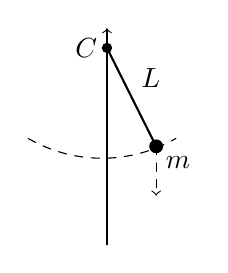
\begin{tikzpicture}[line cap=round,line join=round,scale=2.5]
            \node[left] at (0,1) {\(C\)}; 
            \fill (0,1) circle (0.75pt);

            \draw[-, thick] (0,1) -- (0.25,0.5);
            \fill (0.25,0.5) circle (1pt);
            \node[below right] at (0.25,0.5) {\(m\)}; 
            \node[above right] at (0.125,0.75) {\(L\)}; 

            \draw[->, thin, dashed] (0.25,0.5) -- (0.25,0.25);

            \draw[->] (0,0) -- (0,1.1);
            \draw[dashed] (-0.4,0.54) arc (-120:-60:0.75 and 0.75);
        \end{tikzpicture}
    \end{center}
\end{snippet}

\begin{snippetproposition}{simple-pendulum-equation}{Simple pendulum equation}
    A simple pendulum of length \(L\) subject to a downwards acceleration \(g\) has
    equation
    \[
        \frac{d\theta^2}{dt^2} = -\frac{g}{L}\sin\theta
    \]
    where \(\theta(t)\) is the angular displacement as a \function of time.
\end{snippetproposition}

\begin{snippetproof}{simple-pendulum-equation-forces-proof}{simple-pendulum-equation}{Simple pendulum equation}
    The position of the point is uniquely determined by the radius \(L\) and the angle \(\theta(t)\).
    The force exerted is downwards \(\vec{F} = -mg\hat{z}\). The body is constrained
    by the circular path around the pin. The forces are given by
    \[
        \begin{cases}
            F_N = T - mg\cos\theta \\
            F_T = -mg\sin\theta
        \end{cases}
    \]
    since the tension of the cord \(T\) has no tangential component.
    We know that for any motion, the acceleration can be written as \(\vec{a} = \vec{a_T} + \vec{a_N}\).
    Since \(\vec{a_T} = \frac{dv}{dt}\) and \(\vec{a_N} = \frac{v^2}{R}\),
    \[
        \begin{cases}
            m\frac{v^2}{R} = T - mg\cos\theta \\
            \frac{dv}{dt} = -g\sin\theta
        \end{cases}
    \]
    In this case, the curvature radius \(R\) is precisely the radius of the circle \(R=L\).
    The distance is given by \(s = L\Delta \theta\) and thus
    \[
        v(t) = L\frac{d\theta}{dt}
    \]
    By substituting, we find the tension of the cord as a \function of \(\theta\), which is given by the second equation:
    \[
        \begin{cases}
            T = mL {\left(\frac{d\theta}{dt}\right)}^2 + mg\cos\theta \\
            \frac{d\theta^2}{dt^2} = -\frac{g}{L} \sin\theta
        \end{cases}
    \]
    Note that the first term of the tension is null at the two extremes. The other term becomes
    negative when the ball is in the above semi circumference. Indeed, in such case the tension is negative,
    and the cord exerts tension opposite respect to the other case, as it needs to contract the attempt by the ball
    to crush it. If the the initial velocity is sufficiently high, the tension is still positive if
    the ball is at the top of the circumference (as when it performs a complete turn), in
    that case the ball is still trying to stretch the cable.
\end{snippetproof}

\subsection{Approximations}

\begin{snippetproposition}{simple-pendulum-equation-approx}{Simple pendulum small oscillations}
    A simple pendulum of length \(L\) subject to a downwards acceleration \(g\)
    and small oscillations has equation
    \[
        \theta(t) = \theta_0 \cos\left(\sqrt{\frac{g}{L}}t\right)
    \]
    where \(\theta(t)\) is the angular displacement as a \function of time.
\end{snippetproposition}

\begin{snippetproof}{simple-pendulum-equation-approx-proof}{simple-pendulum-equation-approx}{Simple pendulum small oscillations}
    If we assume small oscillations, we have \(\theta(t) \asymptotic \sin(\theta(t))\), and the equation becomes
    \[
        \frac{d\theta^2}{dt^2} = -\frac{g}{L}\theta
    \]
    which gives the solution
    \[
        \theta(t) = \theta_0 \cos\left(\sqrt{\frac{g}{L}}t + \varphi\right)
    \]
    Since there is no initial velocity, \(\varphi=0\).
\end{snippetproof}

\end{document}
